% Competitive Programming Bootcamp Beamer Template
% Compile with: pdflatex cp_bootcamp_beamer_template.tex
% No shell-escape required.

\documentclass[aspectratio=169,11pt]{beamer}

% ------------------------------------------------------------
% Packages
% ------------------------------------------------------------
\usepackage[utf8]{inputenc}
\usepackage[T1]{fontenc}
\usepackage{lmodern}
\usepackage{amsmath,amssymb,mathtools}
\usepackage{booktabs}
\usepackage{array}
\usepackage{xcolor}
\usepackage{listings}
\usepackage{tikz}
\usetikzlibrary{arrows.meta,positioning,shapes.geometric}

% ------------------------------------------------------------
% Theme setup
% ------------------------------------------------------------
\definecolor{CPNavy}{HTML}{172033}
\definecolor{CPBlue}{HTML}{2563EB}
\definecolor{CPGreen}{HTML}{16A34A}
\definecolor{CPOrange}{HTML}{F97316}
\definecolor{CPRed}{HTML}{DC2626}
\definecolor{CPGray}{HTML}{64748B}
\definecolor{CPLight}{HTML}{F8FAFC}
\definecolor{CPCodeBg}{HTML}{F1F5F9}

\usetheme{default}
\usefonttheme{professionalfonts}
\setbeamertemplate{navigation symbols}{}
\setbeamertemplate{itemize item}{\color{CPBlue}$\blacktriangleright$}
\setbeamertemplate{itemize subitem}{\color{CPGray}$\triangleright$}
\setbeamertemplate{enumerate item}{\color{CPBlue}\insertenumlabel.}

\setbeamercolor{normal text}{fg=CPNavy,bg=white}
\setbeamercolor{frametitle}{fg=white,bg=CPNavy}
\setbeamercolor{title}{fg=white,bg=CPNavy}
\setbeamercolor{subtitle}{fg=CPLight,bg=CPNavy}
\setbeamercolor{block title}{fg=white,bg=CPBlue}
\setbeamercolor{block body}{fg=CPNavy,bg=CPLight}
\setbeamercolor{alerted text}{fg=CPRed}

% Frame title bar
\setbeamertemplate{frametitle}{%
  \nointerlineskip%
  \begin{beamercolorbox}[wd=\paperwidth,ht=0.92cm,dp=0.25cm,leftskip=0.55cm,rightskip=0.4cm]{frametitle}
    \usebeamerfont{frametitle}\insertframetitle\hfill\small\insertframenumber/\inserttotalframenumber
  \end{beamercolorbox}%
}

% Title page
\setbeamertemplate{title page}{%
  \begin{tikzpicture}[remember picture,overlay]
    \fill[CPNavy] (current page.south west) rectangle (current page.north east);
    \fill[CPBlue] ([xshift=-1.4cm,yshift=-1.2cm]current page.north east) circle (2.7cm);
    \fill[CPOrange] ([xshift=0.6cm,yshift=0.2cm]current page.south west) circle (2.2cm);
  \end{tikzpicture}
  \vspace{1.2cm}
  {\color{white}\Huge\bfseries\inserttitle\par}
  \vspace{0.3cm}
  {\color{CPLight}\Large\insertsubtitle\par}
  \vfill
  {\color{CPLight}\large\insertauthor\par}
  \vspace{0.1cm}
  {\color{CPLight}\insertdate\par}
}

% Footer
\setbeamertemplate{footline}{%
  \leavevmode%
  \hbox{%
    \begin{beamercolorbox}[wd=.5\paperwidth,ht=2.4ex,dp=1ex,leftskip=.5cm]{author in head/foot}%
      \color{CPGray}\insertshorttitle
    \end{beamercolorbox}%
    \begin{beamercolorbox}[wd=.5\paperwidth,ht=2.4ex,dp=1ex,rightskip=.5cm plus1fil]{date in head/foot}%
      \hfill\color{CPGray}\insertshortauthor
    \end{beamercolorbox}%
  }%
}

% ------------------------------------------------------------
% Code style
% ------------------------------------------------------------
\lstdefinestyle{cppstyle}{
  language=C++,
  basicstyle=\ttfamily\scriptsize,
  keywordstyle=\color{CPBlue}\bfseries,
  commentstyle=\color{CPGreen},
  stringstyle=\color{CPOrange},
  numbers=left,
  numberstyle=\tiny\color{CPGray},
  stepnumber=1,
  numbersep=6pt,
  backgroundcolor=\color{CPCodeBg},
  showstringspaces=false,
  tabsize=2,
  breaklines=true,
  frame=single,
  rulecolor=\color{CPGray},
  columns=fullflexible
}

\lstdefinestyle{pythonstyle}{
  language=Python,
  basicstyle=\ttfamily\scriptsize,
  keywordstyle=\color{CPBlue}\bfseries,
  commentstyle=\color{CPGreen},
  stringstyle=\color{CPOrange},
  numbers=left,
  numberstyle=\tiny\color{CPGray},
  backgroundcolor=\color{CPCodeBg},
  showstringspaces=false,
  tabsize=4,
  breaklines=true,
  frame=single,
  rulecolor=\color{CPGray},
  columns=fullflexible
}

% ------------------------------------------------------------
% Reusable slide helpers
% ------------------------------------------------------------
\newcommand{\bigO}[1]{\ensuremath{\mathcal{O}\!\left(#1\right)}}
\newcommand{\code}[1]{\texttt{#1}}

\newenvironment{cpbox}[1]{%
  \begin{block}{#1}
  }{%
  \end{block}
}

\newcommand{\probleminfo}[4]{%
  \begin{columns}[T,onlytextwidth]
    \column{0.25\textwidth}\textbf{Input}\par #1
    \column{0.25\textwidth}\textbf{Output}\par #2
    \column{0.25\textwidth}\textbf{Constraints}\par #3
    \column{0.25\textwidth}\textbf{Target}\par #4
  \end{columns}
}

\newcommand{\complexity}[2]{%
  \vspace{0.2cm}
  \textbf{Time:} \bigO{#1}\hspace{0.7cm}\textbf{Memory:} \bigO{#2}
}

% ------------------------------------------------------------
% Deck metadata
% ------------------------------------------------------------
\title[CP Bootcamp]{Competitive Programming Bootcamp Day 1}
\subtitle{Algorithms, Data Structures, and Problem Solving}
\author[Ryan Pelchat]{Ryan Pelchat}
%\date{\today}
\date{August 2026}

\begin{document}

% ------------------------------------------------------------
\begin{frame}[plain]
  \titlepage
\end{frame}

% ------------------------------------------------------------
\begin{frame}{Today’s Roadmap}
  \begin{enumerate}
    \item Problem-solving workflow
    \item Key data structure or algorithm
    \item Worked example
    \item Implementation patterns
    \item Practice problems
  \end{enumerate}
\end{frame}

% ------------------------------------------------------------
\begin{frame}{Bootcamp Problem-Solving Loop}
  \begin{center}
    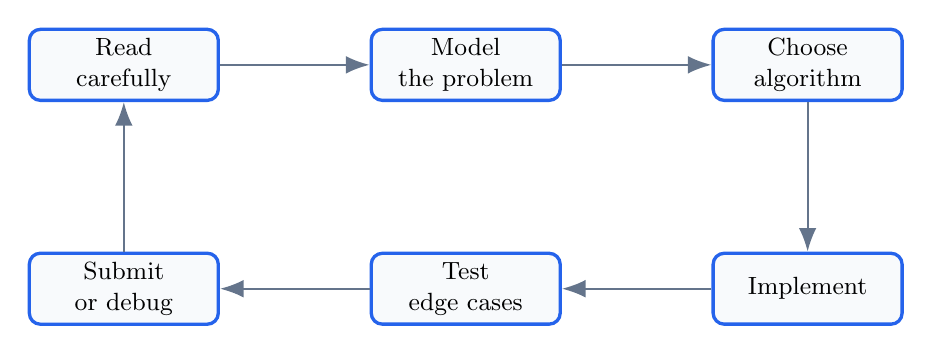
\begin{tikzpicture}[
        node distance=1.9cm,
        every node/.style={font=\small},
        box/.style={rounded corners,draw=CPBlue,very thick,align=center,minimum width=2.4cm,minimum height=0.9cm,fill=CPLight},
        arrow/.style={-{Latex[length=3mm]},thick,draw=CPGray}
      ]
      \node[box] (read) {Read\\carefully};
      \node[box,right=of read] (model) {Model\\the problem};
      \node[box,right=of model] (algo) {Choose\\algorithm};
      \node[box,below=of algo] (code) {Implement};
      \node[box,left=of code] (test) {Test\\edge cases};
      \node[box,left=of test] (submit) {Submit\\or debug};

      \draw[arrow] (read) -- (model);
      \draw[arrow] (model) -- (algo);
      \draw[arrow] (algo) -- (code);
      \draw[arrow] (code) -- (test);
      \draw[arrow] (test) -- (submit);
      \draw[arrow] (submit) -- (read);
    \end{tikzpicture}
  \end{center}
\end{frame}

% ------------------------------------------------------------
\begin{frame}{Problem Slide Template}
  \textbf{Problem:} Replace this with the problem name.

  \vspace{0.35cm}
  \probleminfo
  {Array of $n$ integers}
  {One answer}
  {$1 \le n \le 2\cdot 10^5$}
  {$\bigO{n\log n}$ or better}

  \vspace{0.45cm}
  \begin{cpbox}{Key Observation}
    State the idea that makes the problem easier. For example: sort first, use prefix sums, turn it into a graph, or maintain an invariant.
  \end{cpbox}
\end{frame}

% ------------------------------------------------------------
\begin{frame}{Algorithm Template}
  \begin{enumerate}
    \item Preprocess the input.
    \item Maintain the right state while scanning.
    \item Update the answer greedily / dynamically / using a data structure.
    \item Prove the invariant and analyze complexity.
  \end{enumerate}

  \complexity{n\log n}{n}
\end{frame}

% ------------------------------------------------------------
\begin{frame}[fragile]{C++ Implementation Template}
\begin{lstlisting}[style=cppstyle]
#include <bits/stdc++.h>
using namespace std;

using ll = long long;

int main() {
    ios::sync_with_stdio(false);
    cin.tie(nullptr);

    int n;
    cin >> n;

    vector<int> a(n);
    for (int &x : a) cin >> x;

    // TODO: solve the problem

    cout << 0 << '\n';
    return 0;
}
\end{lstlisting}
\end{frame}

% ------------------------------------------------------------
\begin{frame}[fragile]{Python Implementation Template}
\begin{lstlisting}[style=pythonstyle]
import sys

def solve() -> None:
    input = sys.stdin.readline
    n = int(input())
    a = list(map(int, input().split()))

    # TODO: solve the problem

    print(0)

if __name__ == "__main__":
    solve()
\end{lstlisting}
\end{frame}

% ------------------------------------------------------------
\begin{frame}{Proof Template}
  \begin{cpbox}{Invariant}
    After processing the first $i$ elements, our data structure contains exactly the information needed to answer queries involving those elements.
  \end{cpbox}

  \begin{cpbox}{Why it works}
    Use induction: show that the invariant is true initially, remains true after each update, and implies the final answer.
  \end{cpbox}
\end{frame}

% ------------------------------------------------------------
\begin{frame}{Practice Problems}
  \begin{tabular}{@{}lll@{}}
    \toprule
    Topic & Easy & Medium \\
    \midrule
    Prefix sums & Static Range Sum & Haybales \\
    Greedy & Interval Scheduling & Dragon of Loowater \\
    Graphs & BFS Grid & Shortest Path \\
    DSU & Union Find & Virtual Friends \\
    DP & Fibonacci & Knapsack \\
    \bottomrule
  \end{tabular}
\end{frame}

% ------------------------------------------------------------
\begin{frame}{Recap}
  \begin{itemize}
    \item Identify constraints before choosing an algorithm.
    \item Look for transformations: sorting, graphs, prefix sums, DP states.
    \item Write down the invariant before coding.
    \item Test tiny cases, edge cases, and worst cases.
  \end{itemize}
\end{frame}

% ------------------------------------------------------------
\begin{frame}[plain]
  \begin{center}
    {\Huge\bfseries Questions?}

    \vspace{0.5cm}
    {\Large Let’s solve problems.}
  \end{center}
\end{frame}

\end{document}
